\begin{figure}[tbp]
\centering
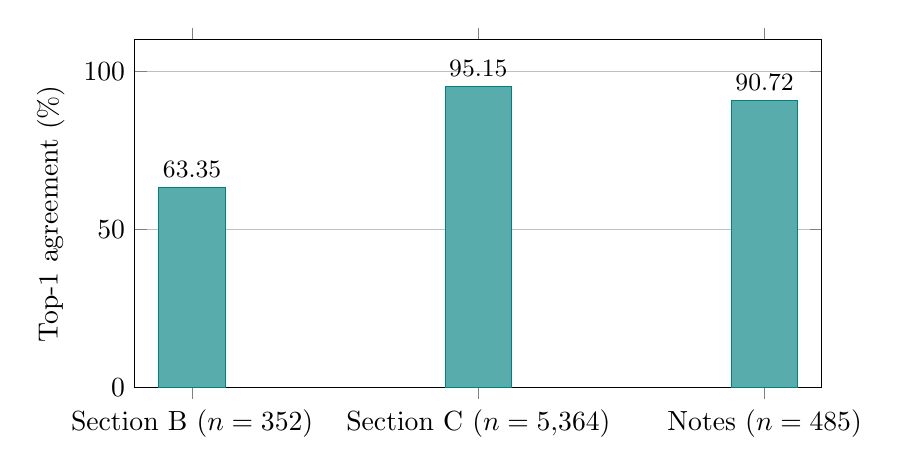
\begin{tikzpicture}
\begin{axis}[width=0.85\linewidth,height=6cm,ybar,bar width=24pt,
  ylabel={Top-1 agreement (\%)},ymin=0,ymax=110,
  symbolic x coords={B,C,Notes},xtick=data,
  xticklabels={Section B ($n=352$),Section C ($n=5{,}364$),Notes ($n=485$)},
  ymajorgrids=true,nodes near coords,nodes near coords style={font=\small},
  point meta=explicit symbolic]
\addplot[fill=teal!65,draw=teal] coordinates {(B,63.35) [63.35] (C,95.15) [95.15] (Notes,90.72) [90.72]};
\end{axis}
\end{tikzpicture}
\caption{Principle-label agreement by source. The bars compare explicitly tagged passages, concept-mapped passages, and principle notes using the filing-derived reference labels. Table~\ref{tab:source} gives confidence intervals calculated by resampling companies.}
\label{fig:source}
\end{figure}
